\documentclass{ieeeaccess}
\usepackage{cite}
\usepackage{amssymb,amsfonts}
\usepackage{algorithmic}
\usepackage{graphicx}
\usepackage{textcomp}
\usepackage{changes}
\usepackage{subcaption}
\usepackage{xcolor}
\usepackage{color, soul}
\usepackage{amsmath}
\usepackage{booktabs}
\usepackage{multirow}

\def\BibTeX{{\rm B\kern-.05em{\sc i\kern-.025em b}\kern-.08em
    T\kern-.1667em\lower.7ex\hbox{E}\kern-.125emX}}
\graphicspath{{image/}}
\makeatletter
\def\endthebibliography{%
	\def\@noitemerr{\@latex@warning{Empty `thebibliography' environment}}%

}
\makeatother


\begin{document}
\history{Date of publication xxxx 00, 0000, date of current version xxxx 00, 0000.}
\doi{10.1109/ACCESS.2017.DOI}

\title{WSNNet: Stacked Bidirectional LSTM with Residual Attention for Indoor Localization of Wireless Sensor Network}
\author{\uppercase{HYUNGTAE LIM}\authorrefmark{1}, \IEEEmembership{Student Member, IEEE},
	\uppercase{CHANGGYU PARK}\authorrefmark{1}, \IEEEmembership{Student Member, IEEE},
	\uppercase{ and Hyun Myung}.\authorrefmark{1},
	\IEEEmembership{Senior Member, IEEE}}
\address[1]{Urban Robotics Laboratory, Korea Advanced Institute of Science and Technology, Daejeon 34141, South Korea.}

\tfootnote{This material is based upon work supported by the Ministry of Trade, Industry \& Energy(MOTIE, Korea) under Industrial Technology Innovation Program. No.10067202, 'Development of Disaster Response Robot System for Lifesaving and Supporting Fire Fighters at Complex Disaster Environment'.}

\markboth
{Author \headeretal: Preparation of Papers for IEEE TRANSACTIONS and JOURNALS}
{Author \headeretal: Preparation of Papers for IEEE TRANSACTIONS and JOURNALS}

\corresp{Corresponding author: Hyun Myung (hmyung@kaist.ac.kr).}

\begin{abstract}
	

As verified experimentally, this new proposal represents a significant improvement in accuracy, computation time, and robustness against outliers.

\end{abstract}

\begin{keywords}
Enter key words or phrases in alphabetical 
order, separated by commas. For a list of suggested keywords, send a blank 
e-mail to keywords@ieee.org or visit \underline
{http://www.ieee.org/organizations/pubs/ani\_prod/keywrd98.txt}
\end{keywords}

\titlepgskip=-15pt

\maketitle

\section{Introduction}
\label{sec:introduction}

\PARstart{W}{ireless} sensor networks(WSN) signifies a number of the sensors which send and receive the signal each other. In recent years, advancement in micro-electo-mechanical systems(MEMS) contributes improvement of sensors' performance and miniaturization at the same time in such a way as to have enabled the wireless sensors to communicate with other wiresless sensors efficiently and conveniently.  By virtue of this low-cost, small-size and acceptively accurate performance, WSNs are widely utilized in various areas, such as resque works, surveillance, pollution monitoring, inspection of structures, and so on\cite{li2009ern,khedo2010wireless,zhang2011indoor,kulaib2011overview}.  

Especially, WSNs are also employeed in various location-aware applications, e.g., tracking and localization of objects. Because WSNs can be easily installed, they have been suggested as a solution for localization on the indoor environment\cite{peneda2009trilateration, jung2011indoor} where the signals of the Global Positioning Systems(GPS) cannot be received. WSNs consist of two types of nodes: anchor nodes(ANs) that interchange signals to tag nodes(TNs) for estimating positions of TNs and TNs whose position are estimated by the gathered data. Several methods for localizing TNs are have been proposed and these are broadly categorized into two categories based on whether the range between the ANs and TNs are measured or not. One method, called range-based, is to directly measure the anchor-to-tag distance or angle, e.g., time of arrival(TOA)\cite{kaune2012accuracy}, time difference of arrival(TDOA)\cite{singh2013tdoa}, time of flight(TOF)\cite{jung2011indoor}, arrival of angle(AOA)\cite{douganccay2008optimal} and the other method is to calcualate position of the TNs using connectivities of the WSNs, e.g., hop counts\cite{banihashemian2018new} or weighted centroid\cite{blumenthal2007weighted}. Usually,   range-based method mostly have better performance than range-free method\cite{han2010pattern} and particularly, TOF-based technique is commonly used in practice because it does not need to synchronize, and is easy to emplement, and consume less resources than other approaches\cite{li2017novel}   

However, these range-based approaches suffer from \textit{rank dificiency} problem, \cite{fabresse2018efficient}, which means range measurements only consist of single value to represent distance between each TN and AN respectively in such a way as to be deficient to describe exact position or orientation of the MNs. Besides, only single value could represent the range measurement, these measurements have huge uncertainties caused by non-line-of-sight(NLOS) problem and multipath fading channel(MPF) problem\cite{li2017novel}. To alleviate these issues, many studies are conducted how to localize more precisely. For example, in \cite{li2017novel}, confidence-based intersection method is proposed for robust trilateration method. In \cite{caballero2008particle}, particle filter algorithm is introduced to estimate the position of a MN attached to a aerial robot while suppressing the noise. Also, many machine learning techniques have been introduced: one authors utilized support vector machine(SVM) for localizaiton\cite{tran2008localization, huan2010three, feng2012determination, afzal2014localization}, other author developed method support vector regression(SVR) for localiztion\cite{lee2013new, lee2013novel}. 

In the meantime, as deep learning age has come\cite{lecun2015deep}, WSNs fields also have introduced various kinds of neural network architectures\cite{rahman2009localization, singh2013tdoa, abdelhadi2013efficient, kumar2016localization, banihashemian2018new}. An main advantage of neural networks-based approaches is that the neural networks enables themselves to recognize the position of the MNs quite accurately through the training even if there is no mathematical description. The neural networks also cover all noises that occurs when ANs and MNs interchange their signals. The authors show that their nerual networks-based approach have better performance than traditional approaches or machine learning-based approaches, yet most networks are based on The Multilayer Perceptron(MLP). In addition, the some authors just show the feasibility of their approaches, i.e., they trained and tested on the simulations situation. Plus, some authors let the neural networks infer the estimates on the two-dimensional space, but gap of the complexity of estimating position between on two-dimensional space and on three-dimensional using \textit{rank-deficient} measurements cannot be negligible.

In this paper, we propose a stacked bidirectional Long Short-Term Memory(stacked Bi-LSTM) with residual attention for more accurate localization of a MN. Our contributions can be summarized as follows. First of all, Using deep learning, our structure directly learns the end-to-end mapping between range data measured by ANs-to-MN distances and the position of MN on three dimensional space. Unlike other approaches whose authors implement MLP-based neural networks, we exploit LSTM architecture in such a way as not only to take present range data but also take previous temporal data as input for estimating the MN's position. Second, we verify that effect of the residual attention in the way that the residual attention layer makes the network better understand context of the feature when dealing with low-dimensional input. Finally, we implement the networks presented at related works and compare which neural architecture perperforms better when real-world data are given as input. As a result, and our networks perform the best performance among other proposed approaches. Our system overview is shown in the figure \ref{fig:system_overview}. 

%실험했다 얘기할 떄


\begin{figure}[h]
	\centering
	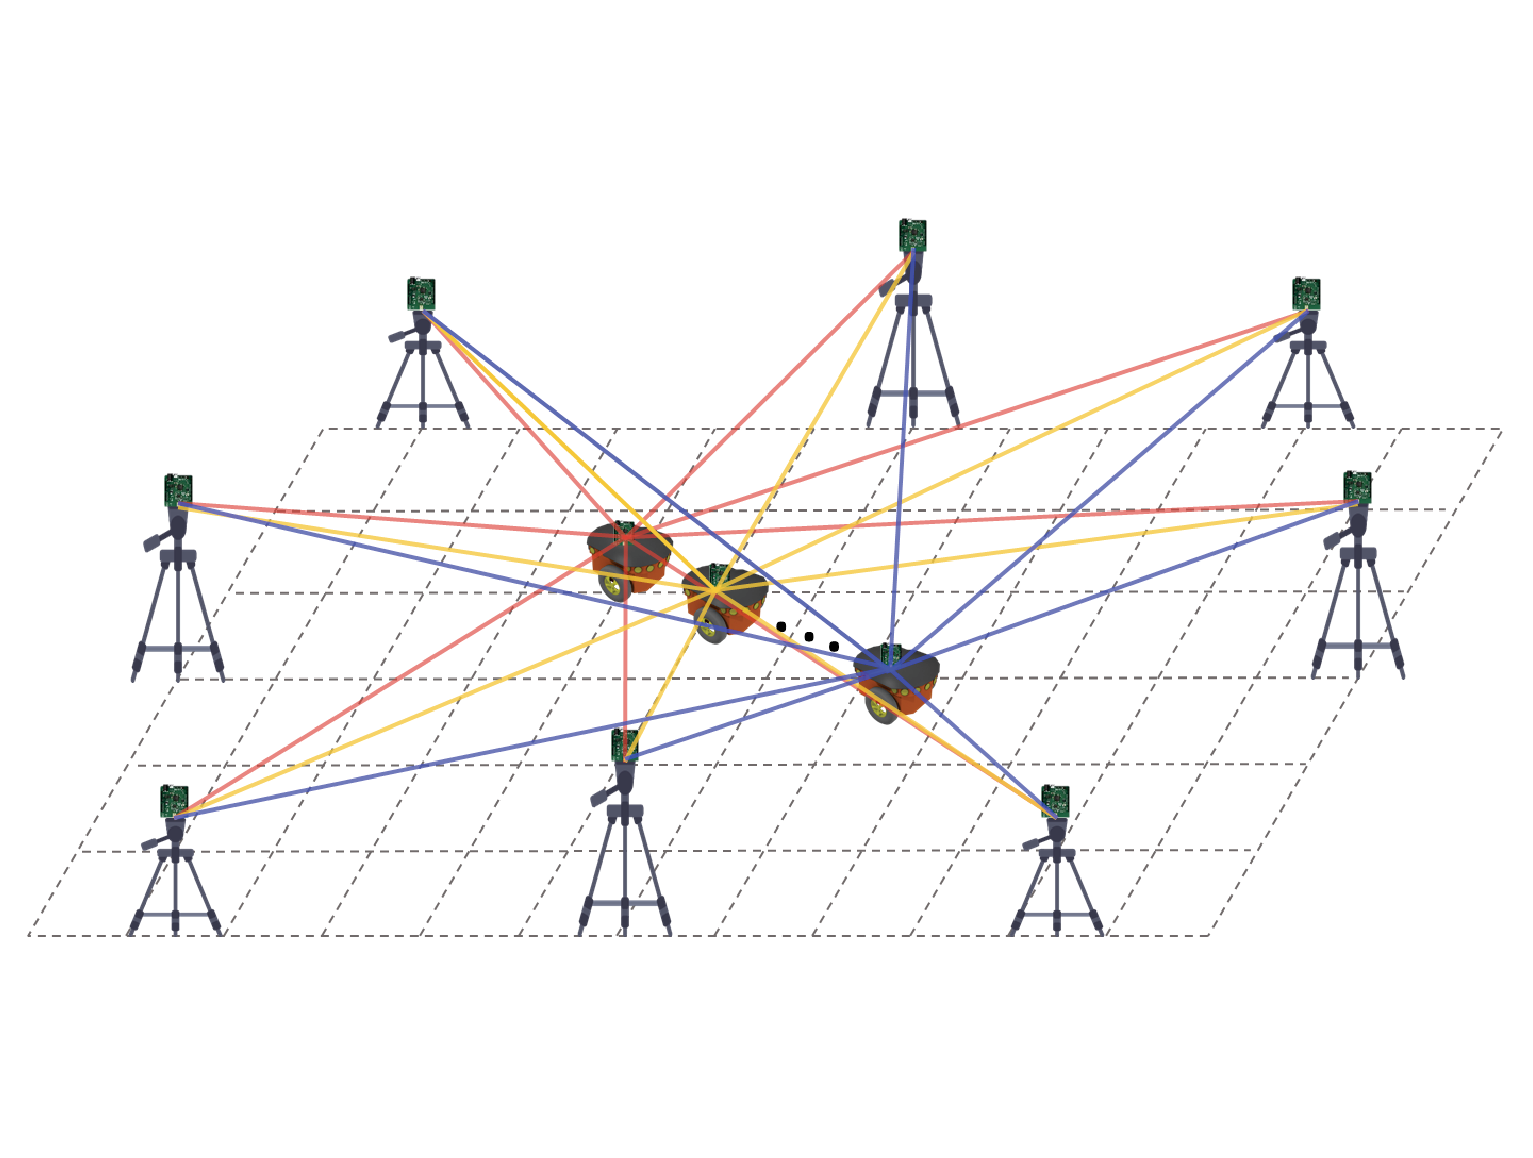
\includegraphics[width=.5\textwidth]{image/Access_overview_figure_1}
	\caption{System overview.}
	\label{fig:system_overview}
\end{figure}

\section{Related Works}

In the past few years, researchers have conducted the studies using machine learning-based approaches to reduce computational complexity and localize a mobile node more precisely. One authors utilized support vector machine(SVM) for localizaiton, \cite{tran2008localization, huan2010three, feng2012determination, afzal2014localization}, other author developed method support vector regression(SVR) for localiztion\cite{lee2013new, lee2013novel}. In \cite{tran2008localization}, authors suggested two SVMs for localization, called LSVMs, one LSVM infers x-dimension and the other LSVM infers y-dimension. To employeeing LSVMs, they divide the field into \textit{M-l} x-classes and \textit{M-l} y-classes, like grid, and this deployment has had an impact on succeeding studies\cite{chatterjee2010fletcher, feng2012determination, afzal2014localization}. Samadian \textit{et al.}\cite{samadian2011probabilistic} introduced probablistic support vector machine for localization and they showed that probablistic vector machine has better performance than LSVM. In terms of SVR, Lee \textit{et al.} suggested various types of SVR for localization\cite{lee2013new, lee2013novel}  

Especially, several works have been studied using neural networks to localize nodes of the range measurement sensors on the indoor space while covering range measurements' uncertainties. Regarding previous proposals, Chenna \textit{et al.} first shows the suitability that Kalman filter could be replaced with the RNN when estimating states and tracking nodes\cite{chenna2004state}. However, they did not provide numerical analysis, so Shareef \textit{et al.} did and conducted their experiment in the real-world. They concluded Radial Basis Function(RBF) may be the best option among the suggested Kalman filter models and RNN\cite{shareef2008localization}. 


\begin{table*}[ht]
	\centering
	\caption{Comparison of previous studies with our approach}
	\begin{tabular}{l|l|l|l|l|l}
		\toprule
		\multicolumn{1}{c}{\textbf{Localization method}} & \multicolumn{1}{c}{\textbf{Dimension}} & \multicolumn{1}{c}{\textbf{Type of input}} & \multicolumn{1}{c}{\textbf{Train data}} & \multicolumn{1}{c}{\textbf{Test data mobility}} & \multicolumn{1}{c}{\textbf{Implementation environment}} \\ 
		\midrule
		RBF\cite{shareef2008localization}                          & \multicolumn{1}{c}{2D}                 & \multicolumn{1}{c}{Temporary}                        & \multicolumn{1}{c}{Grid}                & 
		\multicolumn{1}{c}{Dynamic nodes \checkmark}                & \multicolumn{1}{c}{Real-world \checkmark}                          \\ 
		MLP\cite{rahman2009localization}&        \multicolumn{1}{c}{2D}              &      \multicolumn{1}{c}{Temporary}                                            &   \multicolumn{1}{c}{Grid}                      & \multicolumn{1}{c}{Static nodes}                     &   \multicolumn{1}{c}{Simulation}    \\ 
		
		MLBPN\cite{singh2013tdoa}&
		\multicolumn{1}{c}{2D}                   &      
		\multicolumn{1}{c}{Temporary}                 &   \multicolumn{1}{c}{Grid}                   & 
		\multicolumn{1}{c}{Static nodes}        &   \multicolumn{1}{c}{Simulation}   \\ 
		
		MLP\cite{abdelhadi2013efficient}& 
		\multicolumn{1}{c}{3D  \checkmark}                   &      
		\multicolumn{1}{c}{Temporary}                 &   \multicolumn{1}{c}{Spread \checkmark}                   & 
		\multicolumn{1}{c}{Static nodes}        &   \multicolumn{1}{c}{Simulation}   \\ 
		
		c-FCNNs\cite{bernas2015fully}& 
		\multicolumn{1}{c}{2D}                   &      
		\multicolumn{1}{c}{Temporary}                 &   \multicolumn{1}{c}{Spread \checkmark}                   & 
		\multicolumn{1}{c}{Static nodes}        &   \multicolumn{1}{c}{Real-world  \checkmark}   \\ 
		
		MLP\cite{kumar2016localization}& 
		\multicolumn{1}{c}{2D}                   &      
		\multicolumn{1}{c}{Temporary}                 &   \multicolumn{1}{c}{Grid}                   & 
		\multicolumn{1}{c}{Static nodes}        &   \multicolumn{1}{c}{Real-world  \checkmark}   \\ 
		LPSONN\cite{banihashemian2018new}&     
		\multicolumn{1}{c}{2D}                   &      
		\multicolumn{1}{c}{Temporary}                 &   \multicolumn{1}{c}{Spread  \checkmark}                   & 
		\multicolumn{1}{c}{Static nodes}        &   \multicolumn{1}{c}{Simulation}   \\ 
		
		Ours&
		\multicolumn{1}{c}{3D \checkmark}                   &      
		\multicolumn{1}{c}{Sequential \checkmark}                 &   \multicolumn{1}{c}{Spread \checkmark}                   & 
		\multicolumn{1}{c}{Dynamic nodes \checkmark}        &   \multicolumn{1}{c}{Real-world \checkmark}   \\ 
		\bottomrule
	\end{tabular}
	\label{table:related_worsk}
	
\end{table*}

\begin{figure*}[h]
	\centering
	\includegraphics[width=.9\textwidth]{image/networks}
	\caption{Our proposed network architecture.}
	\label{fig:our_network}
\end{figure*}

Similarly, many researchers also have achived considerable improvement to localize position of mobile node by exploiting MLP in WSNs fields\cite{shareef2008localization, rahman2009localization, singh2013tdoa,abdelhadi2013efficient,bernas2015fully, kumar2016localization, banihashemian2018new}. In case of range-based method, Rahman \textit{et al.} \cite{rahman2009localization} have considered the neural networks for mapping between RSS and corresponding position of sensor nodes and let neural networks be trained by the train data gathered by the sensor nodes that are eqaully spaced over x-axis and y-axis. In \cite{singh2013tdoa}, Singh \textit{et al.} compared that performance of Multilayer Back propagation Network Model(MLBPN) and Radial Basis Function Network Model(RBFN) and the authors show that RBFN performs better than MLBPN when the number of the sensor nodes is larger than 220. Abdelhadi \textit{et al.}  \cite{abdelhadi2013efficient} presented two artificial intelligence techniques: Sugeno-type fuzzy system and neural networks system. In addition, the authors conducted experiment on three-dimensional space in such a way as verified the feasibility of localization by utilizing nueral networks in 3D space. Kumar \textit{et al.} \cite{kumar2016localization} also introduced the neural networks and evaluated five different training techniques,e.g., Levenberg-Marquardt (LM), Bayesian Regularization
(BR), Resilient Back-propagation (RP), Scaled Conjugate Gradient (SCG) and Gradient
Descent (GD), to find optimal way to train neural networks with the best accuracy. Recently, \cite{banihashemian2018new} have proposed the neural networks with novel training technique, called Particle Swarm Optimization(PSO) and prove thire nerwork, called LPSONN, has better localization accuracy than previous machine learning method, soft computing method, and previously proposed network.




However, there are some points that could have been better. First of all, in some cases, their networks were trained by range measurement data corresponding position of mobile node in simulation environment\cite{chatterjee2010fletcher, shareef2008localization, rahman2009localization, singh2013tdoa, banihashemian2018new}. The simulation situation is almost ideal in the point that the NLOS or MPF problem does not occur. Even though in \cite{rahman2009localization}, they artificially generate NLOS data, but the gap of complexity between real-world and artificially generated data exists, since the generated data has less noise than those of real-world necessarily. For these reasons, it is hard to say that their networks also works well on real world situation. Therefore, to test on whether it is possible for neural networks to estimate position with covering all disturbance, the experiment should be conducted on real-world. 
Second, some studies was conducted on the two-dimensional space to simplify their problem definition\cite{shareef2008localization, rahman2009localization, singh2013tdoa,bernas2015fully, kumar2016localization, banihashemian2018new}. However, gap of the complexity of estimating position between on two-dimensional space and on three-dimensional using \textit{rank-deficient} measurements cannot be negligible. Finally, in previous studies \cite{shareef2008localization, rahman2009localization, singh2013tdoa,kumar2016localization}, it has a possibility of overfitting because the authors generate the grid-map as train data in such a way as to restrict their ground truth region. That is to say, their finite groud truth indicates where the sensors are placed at the equal distance interval so that nerual networks may recognize the only locations included in the grid are correct even when the position of MN to be tested is quite far from the grid. Therefore their grid map train impedes the optimization of nueral netorks to cover all over the region.

%그들이 제시한 test data에서 성능이 좋을 수 있을ㅈ지 몰라도, 조금만 바꾸게 되면 성능이 떨어질 수 도 있음
%채워지지 못 한 부분
%그리고 노이즈가 발생했을 시에는 같은 포지션이었더라도 값이  많이 달라 질 수 있음
%
%진행 중 
 
%대부분의 연구 결과가 2D상에서 진행되었는데, 이것은 오히려 noise가 발생했을 때 숨기는 거임!

%격자로 나뉨 - 움직인다면 움직이지 않은 부분에 대해서는 학습을 하지 못하므로 정확성이 떨어짐
%대체로 simulation: 하지만 simulation의 상황에서는 실제의 데이터에서 일어나는 noise들이 비교적 적음. 좀더 complex하지 않은 ideal 상황임
%2D




%analogous: 유사한

%Localization Using Neural Networks in Wireless Sensor Networks \cite{shareef2008localization} - 변화되는 위치에 대응되는 걸 학습한 게 아니라 x,y,z에 대한 3개의 beacon의 l을 finger print map 방식으로 학습한거지! x,y만 추정  grid를 나눠서 모든 공간에 대한 거리에 대한 위치를 finger print 기법

%Localization of Wireless Sensor Network using artificial neural network \cite{rahman2009localization}
%TDOA Based Node Localization in WSN using Neural Networks \cite{singh2013tdoa} 2D simulation sequential x MLP ,RBF
%Efficient Artificial Intelligent-based Localization Algorithm for Wireless Sensor Networks \cite{abdelhadi2013efficient} : 3D random하게 뿌리지만 simulation sequential modeling을 하지 않음! MLP

%Blanco \textit{et al.} suggest two methods: one method is to employee Rao-blackwellized particle filter(RBPF), which divide one hidden state into the state of landmarks and the state of robot so that variance could be reduced \cite{blanco2008pure}, and the other is to e exploiting the conditional independence between the position distributions of  each beacon within a Rao-Blackwellized Particle Filter (RBPF)  for maintaining independent Sum of Gaussians (SOGs) for  each beacon \cite{blanco2008efficient}  



%Ideal case에서 배치를 같은 높이에 두었을 때는 수식이 A는 full rank가 아니어서  역행렬이 존재하지 않는다. 하지만 real-world에서는 미세한 error가 발생하기 때문에, 
%만약 full rank 여서 역행렬이 존재한다고 하면 역행렬을 구하는 과정에서 A-1의 값이 엄청 커지게 됨!

\section{WSN Net}

In this chapter, we explain how our proposed residual attention-based stacked Bi-LSTM is implemented, as illustrated in Fig. \ref{fig:our_network}. 
In detail, we introduce the neural networks concepts that we choose for localizaing the tag node and the describe the reason why we let the neural network infer in three-dimensional space even though experiment is conducted on the mobile robot. Finally, we explain how to set the loss function of our neural network and then compare to those of other previous works.


\subsection{long short-Term Memory}


Recurrent Neural Networks(RNN) is a special artificial neural networks in the way that it has a loop, so that RNN can deal with temporal information for sequential modeling. It originally used in the natural language processing, speech recognition, and image captioning area. By virtue of a loop, RNN can remember past data and past situation and respond appropriately to the present situation based on these past information. 

But unfortunately, as the time-sequential gap grows, RNNs become unable to learn the relationship of these sequential information. This issue is called the problem of \textit{Long-Term Dependency},which fail to propagate the previous matter into present tasks so that long-term dependency lead to a failure of learning. In other words, RNNs are not able to learn to store appropriate internal states and operate on long-term trends. That is the reason why the Long Short-Term Memory (LSTM) architecture is introduced to solve this long-term dependency problem and make the networks possible to learn longer-term contextual
understandings \cite{hochreiter1997long}. That's why LSTM have been actively studied for many tasks in a wide area of science and engineering.in most of the deep learning research areas and numerous variations of LSTM architecutres have been studied.

\begin{figure}[h]
	\centering
	\includegraphics[width=.4\textwidth]{image/basic_LSTM_revised}
	\caption{Architecture of the LSTM. It consists of 3 gates, forget gate(the part inside the red box), input gate(the part inside the blue box), and output gate. And output gate is divided into cell state layer(the part inside the green box) and output gate layer(the part inside the cyan box) 
	}
	\label{fig:basic_lstm}
\end{figure}

Unlike RNN that consist only of hidden state, in LSTM, cell state is added on the network. The cell state consists of the 3 gates to preserve the previous information and control the cell state: forget gate, input gate, and output gate and equations of those are as follows:




\begin{align}
f_{t} & =\sigma _{s}\big(W_{xf}\cdot x_{t}+W_{hf}\cdot h_{t-1}+b_{f}\big)\label{eq:forget}\\
i_{t} & =\sigma _{s}\big(W_{xi}\cdot x_{t}+W_{hi}\cdot h_{t-1}+b_{i}\big)\label{eq:input}\\
\tilde{c}_{t} & = \tanh\big(W_{xc}\cdot x_{t}+W_{hc}\cdot h_{t-1}+b_{c}\big)\label{eq:new_cell}\\
c_{t} & =f_{t}\odot c_{t-1}+i_{t}\odot\tilde{c}_{t}\label{eq:update}\\
o_{t} & =\sigma _{s}\big(W_{xo}\cdot x_{t}+W_{ho}\cdot h_{t-1}+b_{o}\big)\label{eq:output}\\
h_{t} & =o_{t}\odot \tanh\big(c_{t}\big)\label{eq:hidden}
\end{align}

where $\sigma _{s}$ is a kind of activation function, called \textit{sigmoid},  $f_{t}$, $i_{t}$, and $o_{t}$ respectively indicates the forget gate, input gate, and output gates, and $c_{t}$ denotes cell states. And $\odot$ denotes element-wise multiplication, called \textit{Hadamard product}. Entire gates are activated by sigmoid function and cell states are activated by $\tanh$ function.

The Forget gate layer, $f_{t}$, decides how much information to forget. The sigmoid layer, which is the activation function of $f_{t}$, takes previous hidden state, $h_{t}$, and present input, $x_{t}$ and outputs a number between 0 and 1. Note that 1 indicates "totally keep the previous cell state, $C_{t-1}$" and 0 indicate "totally forget $C_{t-1}$" \eqref{eq:forget}. Next, the input gate, $i_{t}$, decides how much information to embrace when updating the cell state. $i_{t}$ are also from the sigmoid function layer \eqref{eq:input} and $tanh$ generates the new candidate cell state, $\tilde{c}_{t}$, which ranges from -1 to 1 \eqref{eq:new_cell}. After that, $c_{t}$ is updated by the cell state layer based on $f_{t}$, $i_{t}$, and $\tilde{c}_{t}$ \eqref{eq:update}. In addition, output gate layer, $o_{t}$, sereves as a filter, which means $o_{t}$ determine what values are going to output \eqref{eq:output} in such a way as that present hidden state, $h_{t}$, is updated based on $o_{t}$ updated cell state, $c_{t}$ \eqref{eq:hidden}. 


\subsection{Bidirectional LSTM}

\begin{figure}[h!]
	\centering
	\includegraphics[width=.9\linewidth]{bidirectional_LSTM_revised}
	\caption{Architecture of the Bidirectional LSTM(Bi-LSTM)}
	\label{fig:bidirectional_revised}	
\end{figure}


One shortcoming of conventional RNNs is that they only exploit previous context to update $h_{t}$ and $c_{t}$. However, in many cases dealing with sequential data, it could be efficient to extract well-discribed context by utilizing future context as well. Bidirectional RNNs are introduced\cite{schuster1997bidirectional} for that reason and bidirectional RNNs process the data in both directions with two separate hidden layers. Especially, bidirectional LSTM, which we employee, has one forward LSTM and one backward LSTM running in reverse time and their features are combined at the output layer, $y_{t}$. As a result, bidirectional LSTM can produce more appropriate context considering both past and future at the same time. By virtue of this characteristics, bidirectional LSTM is popularly utilized for many tasks to model their sequentional systems \cite{zhang2017multi,li2018human,ullah2018action}. 


As FIGURE. \ref{fig:bidirectional_revised} shown, bidirectional LSTM consist of 2 LSTMs: one forward LSTM layer, $\overrightarrow{LSTM}$, and one backward LSTM layer, $\overleftarrow{LSTM}$. Let assume the hidden state of $\overrightarrow{LSTM}$ at the time step $t$  be $h^{f}_{t}$ and $\overleftarrow{LSTM}$ at the time step $t$  be $h^{b}_{t}$, the hidden states and output sequence, $y_{t}$ are calcaulated as follows:

\begin{align}
h^{f}_{t} & =\overrightarrow{LSTM}\big(x_{t}, h^{f}_{t-1}\big)\\
h^{b}_{t} & =\overleftarrow{LSTM}\big(x_{t}, h^{b}_{t+1}\big)\\
y_{t} & =\sigma _{R}\big(W_{h^{f}y}\cdot h^{f}_{t}+W_{h^{b}y}\cdot h^{b}_{t}+b_{y}\big)
\end{align}

where $\sigma _{R}$ denotes activation function called ReLu. Note that in our case, we concatenate $h^{f}_{t}$ and $h^{b}_{t}$ to preverse their contexts seperately as our range measurement, which is gathered by the tag node and each anchor node, suffer from the \textit{rank-dificiency},which means range-based measurement consist of one-dimensional data\cite{fabresse2013undelayed}. Hence, we judge that it would be more helpful to increase the number of features naturally by concatenating two hidden states rather than adding them and when the network infer the position  .

\subsection{Stacked Architecture}

Recently, researchers show that the deeper the architecture of neural networks, the better their performance\cite{simonyan2014very, he2016deep} and their demonstrations has opened a deep learning area. Likewise, many authors have analyzed variations of LSTM architecture and find out that stacking multiple layers of the LSTM improve the performance for many tasks\cite{graves2013hybrid, graves2013speech,ullah2018action}. In other words, as the number of stacked layers is getting large, the more activation functions which rise the non-linearity within the networks are stacked  in such a way as that complexity of networks increases. As a results, networks could model more complex system by virture of these increased non-linerity.

Therefore, we also construct our networks by stacking two LSTM to increase the non-linearity. Note that stacking more than three LSTM doesn't show the improvement of performance. We suppose that activation funtions within the LSTM cause the \textit{vanishing gradient problem}\cite{pascanu2013difficulty}, which the networks fail to training due to the fact that the gradient is getting closer to zero during the backpropagation. We deem that this problem could comes from the sigmoid function and $tanh$ function that compose the part of LSTM. Consequently, we put the ReLu function between LSTMs to avoid the vanishing gradient problem\cite{nair2010rectified}, instead of stacking LSTM.    

\subsection{Residual Attention layer}

A Attention layer is powerful module nowadays and mostly improves performance of neural network. Originally, neural networks treats information equally. But, using attention layer, neural networks can be ATTENDED what it should be examined closely. At the first time, attention is utilized at natural language processing area for improving translation performance\cite{luong2015effective}. But nowadays, attention layer is employed in many areas to improve the performance of the networks. For example, Jaderbeg \textit{et al.}\cite{jaderberg2015spatial} introduced the attention layer to let the neural networks attend to spatial information. In addition, attention is even utilized to pose estimation and optimization\cite{parisotto2018global}, detection\cite{zhu2018towards}, and video captioning\cite{xu2017learning} 

To precisely estimate the position of the tag node, it is important for the network to distinguish which is more meaningful context on time step \textit{T} to help contextual understanding of our  networks. So, we add the attention layer between the LSTM and the attention layer take on a role of a feature selector\cite{wang2017residual}. The equation of the attention machanism is as follows:  

\begin{equation}
H(x)=M(x)\odot x
\end{equation} 

where $x$ denotes the output of previous neural network layer, $H(x)$ denotes the output of the attention layer to be passed to the next neural network layer and $M(x)$ denotes the attention mask.  The attention layer takes $s$ as input and outputs the $H(x)$. By element-wise multiplying x by $M(x)$, attention layer makes the network weight more crutial information. 

Despite of the improvement of the performance, the attention layer has potential risks that it may dilutes the features because attention mask ranges over 0 to 1. To alleviate this problem, residual attention layer is introduced in our network as follows\cite{wang2017residual}:

\begin{equation}
H(x)=\left(1+M(x)\right)\odot x
\end{equation} 

As blue cuboid shape in the FIGURE \ref{fig:our_network} shown, this idea is originated from the Residual Net(ResNet)\cite{he2016deep} that has skip connection in such a way as to mitigate aforementioned dilution problem and help the network to be trained well. Likewise the ResNet, residual attention also has other branch to calculate how much to attend and the branch is joined with original feature vector $x$. Each hidden state has each residual attention layer so that these attention modules can determine which time stamp has more fruitful meaning and deliver the output to second bidirectional LSTM.


\subsection{Training loss}

  In this section, we describe the method for training our network. Generally, let $n$ be the number of mobile nodes and $m$ be the number of the anchor nodes, data set are represented as follows:
  
  \begin{equation}
  \left\{(l_{11}, l_{12}, ..., l_{1m}, P_1),...,(l_{n1}, l_{n2}, ..., l_{nm}, P_n)\right\}
  \end{equation} 
  
  
 where $l_{ij}$ denotes the the distance between $i^{th}$ mobile node and $j^{th}$ anchor node, $P_i$ denotes the position of mobile node, which consist of 2D ($x$ and $y$), or 3D ($x$,$y$, and $z$). 
 In other words, data consist of set of distance data corresponding to the position of mobile nodes. Conseqeuntly, neural network  could be optimized to be able to localize the mobile node when take distance set as input.
 

 %그들의 문제점
 
 our neural network does not only take a set of distance data but takes sets of distacne data on the time step $T$ where $T$ indicates sequential length of input to our network. And in our case, one mobile node is only placed on the robot. Therefore, data are formulated as follows:
 
 \begin{equation}
 %$L = \left\{(X_t, Y_t)\right \}$ 
 \mathbb{L} = {(L_t, Y_t)} 
 \end{equation}
 where $L_t = \left\{(l_1, l_2... , l_m)_t\right\}$ denotes input range measurement between a tag node end each anchor node at the time $t$. We omit the part of subscript that indicates $i^{th}$mobile node because we have only one mobile node. $Y_t$ denotes the ground truth of the robot's 3D position, which is denoted as $Y_t = \left\{x_t, y_t, z_t\right\}$.
 
 Let $\Theta$ be the parameters of our network model and assume that the trained network model could be expressed as conditional probability as follows:

\begin{multline}
 P(Y_t|L_{t-T+1}, L_{t-T+2},..., L_t) =\\
 p((x_t, y_t, z_t)|(l_1,..., l_m)_{t-T+1},(l_1,..., l_m)_{t-T+2}..., (l_1,..., l_m)_t)
\end{multline}  

Note that other studies only consider the input on time t, yet our approach consider temporal information about the range measurement data. Then, our final goal is to find optimal parameters $\Theta^{*}$ for localization by minimizing $L_2$ loss term. The $L_2$ loss term indicates mean square error(MSE) of Euclidean distance between ground truth position $Y_k$ and estimated position $\hat{Y_k}$ as follows:

\begin{equation}
\Theta^{*} = \underset{\Theta}{\mathrm{argmin}} \frac{1}{N} \sum_{k=1}^N \parallel Y_k - \hat{Y_k} \parallel^{2}
\end{equation}  
 
\subsection{Why on three-dimensional?}

\begin{figure}[h]
	\centering
	\includegraphics[width=.4\textwidth]{image/3D_error_increasing_revised}
	\caption{Figures from experiment (a)The anchor and tag nodes (b)Four examples of the trajectory (c) the process that makes dataset}
	\label{fig:range_error_reason}
\end{figure}

One may ask a question that why we infer the robot's position on the three dimensional space even test are being conducted on the mobile robot. It is true that position of the $z$ varys very little. However, we found that localizing the mobile node on the three dimensional space using range measurement data is very week to noise. In more detail, let assume that 4 anchor node are placed on the ground and form square with similar height. Let $x_i$, $y_i$, $z_i$, and $d_i$ be the position of $i^th$ anchor node and range measurement. Then equations on the 3-D space are as follows:      


\begin{equation}
%\left\(\right\) 
(x-x_1)^2+(y-y_1)^2+(z-z_1)^2={d_1}^2 \label{eq:range1}
\end{equation}
\begin{equation}
(x-x_2)^2+(y-y_2)^2+(z-z_2)^2={d_2}^2 \label{eq:range2}
\end{equation}
\begin{equation}
(x-x_3)^2+(y-y_3)^2+(z-z_3)^2={d_3}^2 \label{eq:range3}
\end{equation}
\begin{equation}
(x-x_4)^2+(y-y_4)^2+(z-z_4)^2={d_4}^2 \label{eq:range4}
\end{equation}

where $x$, $y$, and $z$ is the unkown position of the mobile node. And we can rewrite these equation by substracting \eqref{eq:range4} from \eqref{eq:range1}, \eqref{eq:range2}, and \eqref{eq:range3} 

\begin{equation}
A_{3D}X_{3D}=b_{3D}
\end{equation}

where $X_{3D}$ indicates $[x,y,z]^T$ and $A_{3D}$ and $b_{3D}$ are as follows: 

\begin{equation}
A_{3D} =\left[ {\begin{array}{ccc}
	2(x_2-x_1) & 2(y_2-y_1) & 2(z_2-z_1)\\
	2(x_3-x_1) & 2(y_3-y_1) & 2(z_3-z_1)\\
	2(x_4-x_1) & 2(y_4-y_1) & 2(z_4-z_1)\\
	\end{array} } \right]
\end{equation}

\begin{equation}
b_{3D} = \left[ {\begin{array}{c}
	\substack{
		({d_1}^2-{d_2}^2)-({x_1}^2-{x_2}^2)-({y_1}^2-{y_2}^2)-({z_1}^2-{z_2}^2)\\
		({d_1}^2-{d_3}^2)-({x_1}^2-{x_3}^2)-({y_1}^2-{y_3}^2)-({z_1}^2-{z_3}^2)\\
		({d_1}^2-{d_4}^2)-({x_1}^2-{x_4}^2)-({y_1}^2-{y_4}^2)-({z_1}^2-{z_4}^2)\\
	}
	\end{array} } \right]
\end{equation}

Unlike the case of 2D, $A_{3D}$ consists of $z$ components on the third column. Anchor nodes are placed in a less scattered on the z direction than x and y axis. In other words, it is hard to put the anchor nodes with exactly same height in real-world, which means $z_1\approx z_2\approx z_3\approx z_4$. Consequently, values on the third column of $A_{3D}$ converge to zero. Let assume that $A_{3D}$ be full rank in such a way as to $\exists A_{3D}^{-1}$, then values of third row of $A_{3D}^{-1}$ relatively have considerable nubmers. As a result, this make z value very unstable in such a way as to cause huge error with respect to z adirection. 


\begin{figure}[h]
	\centering
	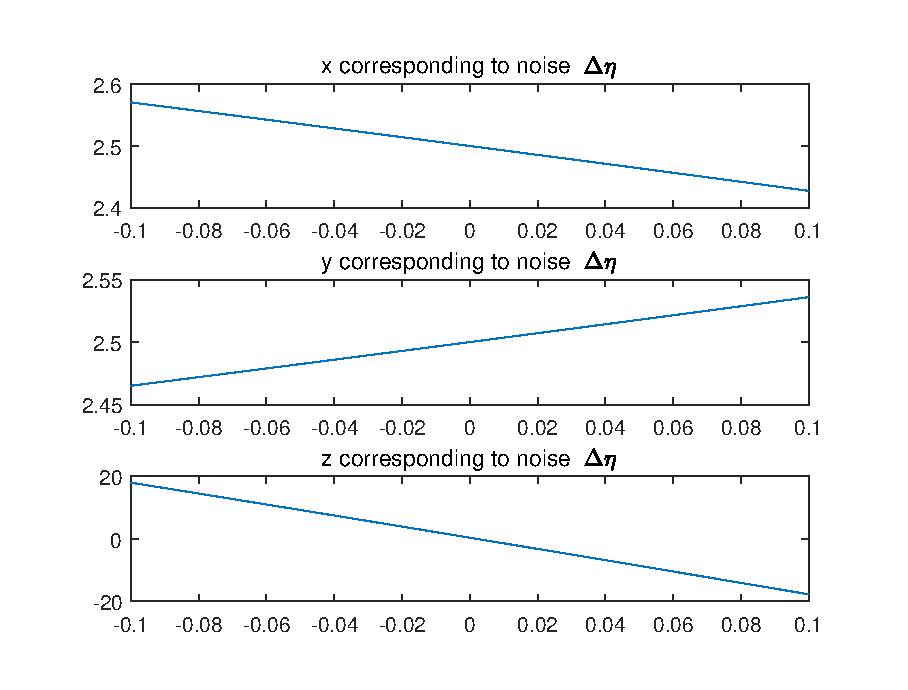
\includegraphics[width=.5\textwidth]{image/noises}
	\caption{(-0.01,0.001, 0.24), (5.02, 0.01, 0.2), (5, 5.01, 0.21), (0.01, 4.999, 0.23) true: (2.5, 2.5,0.4)}
	\label{fig:noise}
\end{figure}


\section{Experiments}
\subsection{Experimental environment}

\begin{figure*}[h]
	\centering
	\begin{subfigure}[b]{.25\textwidth}
		\centering
		\includegraphics[width=.9\textwidth]{anchor_tag_nodes}
		\label{fig:dataset} 	
		\caption{}
	\end{subfigure}%
	\begin{subfigure}[b]{.25\textwidth}
		\centering
		\includegraphics[width=0.9\textwidth]{paths}
		\label{fig:nodes} 	
		\caption{}
	\end{subfigure}%
	\begin{subfigure}[b]{.5\textwidth}
		\centering
		\includegraphics[width=0.9\textwidth]{dataset_process}
		\label{fig:trajectories} 	
		\caption{}
	\end{subfigure}
	\caption{Figures from experiment (a)The anchor and tag nodes (b)Four examples of the trajectory (c) the process that makes dataset}
	\label{fig:experiments}
\end{figure*}
Our experimental system consists of a UWB(ultra wideband) sensor tag node attached on the mobile robot platform and eight anchor nodes that have a UWB transceiver, the motion capture system with 12 cameras, and a small-form-factor(SFF) computer.


\begin{figure}[h]
	\centering
	\includegraphics[width=.4\textwidth]{anchor_tag_nodes}
	\caption{(a)The anchor and tag nodes}
	\label{fig:environment}
\end{figure}


UWB sensor anchors are attached to landmarks. These become the end points of the range measurements. The anchor nodes transmit the UWB signal. A UWB sensor tag is attached to a robot. It becomes the opposite side end point of the measurements. The tag node receives the signal and measures the range between two devices. Each UWB transceiver, DW1000 UWB-chip made by Decawave, supports 6 RF bands from 3.5 GHz to 6.5 GHz. It measures in centimeter-level accuracy. Fig. \ref{fig:experiment} shows anchor and tag nodes.

We inference the position of a robot with our network. To train the network and test the results, the ground truths are needed. We get the ground truth by using the motion capture system. The system is Eagle Digital Realtime system of motion analysis corporation that operates with the principle of stereo pattern recognition that is a kind of photogrammetry based on the epipolar geometry and the triangulation methodology. We attach four markers to a robot. The system gives us the location of these markers and has < 1mm accuracy.

A mobile robot used in experiment is iClebo Kobuki from Yujinrobot that has 70 cm/s maximum velocity.The small form-factor computer is a gigabyte Ultra compact PC. Deep learning framework used for our network is pytorch 0.4.0 on python 3.6. The network inferences on the same setting.

The UWB tag is attached to mobile robot that has a small compact computer. The UWB anchors are attached to stands that have two different heights. The anchors are positioned randomly in the square space. As you can see in Fig. \ref{fig:experiment}(b), a mobile robot manually goes on various random trajectories by experimenters.

During the robot is going on, the data is saved in the computer. The distance data used for input data is measured by the UWB sensors. The global position data used for ground truth is measured by the motion capture system. These two kinds of data are paired in a dataset. The computer receives these two kinds of data respectively and syncronizes these by time. To synchronize, we make an independent thread that concatenates and saves these data at the same time. The data is saved at 20Hz frequency. Each trajectory becomes one dataset. All the trajectories are different. Fig. \ref{fig:experiment}(c) shows this process. After collecting whole datasets, we separate the entire dataset to two types, some are the training datasets and others are test datasets.

\subsection{Data syncronization for Train/Test data}
\subsection{Training the Networks}


\section{Results}

\textcolor{green}{To verify our proposal that RNNs can estimate the robot's position through varying range data, we trained our RNN-based multimodal architecture. Plus, to compare to previous traditional SLAM algorithm, we also estimate robot's position by particle filter(PF) based algorithm.}
\subsection{Performance according to the sequence length}

As illustrated in Experiment session, train data are our own data gathered by UWB sensors and motion capture camera, so neural networks take range-only measurements as input and output robot's position. Ground truth data is robot's position measured by eagle eye motion capturer, whose error is in mm units. The results of trajectory prediction are shown in Fig. \ref{fig:trajectory} and Root-Mean-Squared Error (RMSE) are shown in Table \ref{table:RMSE_table}. Note that out experiment is conducted on mobile robot, so we can pre-estimates that z position of robot is almost similar while robot is running. 

We set two test trajectory cases: an square path and zigzag path. an The results shows that it has better performance than established probabilistic-based approach. In both cases, performance of our networks  is better that of particle filter. RMSE of our networks in test1 is 3.928cm and 4.119cm in test2.

We also verified effectiveness of attention layer. It was confirmed that the performance of the networks with the attention layer is improved compared to the networks without the attention layer.


. We also provide statistical analysis from simulations demonstrating that
our new approach can cope with highly noisy sensors and
reduces in one order of magnitude the average errors of the
method proposed

\begin{table}[h]
	\begin{tabular}{lllcc}
		\hline
		\multicolumn{5}{c}{The results of RMSE{[}cm{]}}                                                                          \\ \hline
		\multicolumn{3}{c|}{Model}                                        & \multicolumn{1}{c|}{Test1}          & Test2          \\ \hline
		\multicolumn{3}{l|}{Particle Filter-based w/o pre-estimates of z} & \multicolumn{1}{c|}{11.253}         & 9.195          \\
		\multicolumn{3}{l|}{Particle Filter-based}                        & \multicolumn{1}{c|}{5.525}          & 5.258          \\
		\multicolumn{3}{l|}{Multimodal(Ours)}                                   & \multicolumn{1}{c|}{4.225}          & 4.311          \\
		\multicolumn{3}{l|}{Multimodal(Ours) + attention}                       & \multicolumn{1}{c|}{\textbf{3.928}} & \textbf{4.119}
	\end{tabular}
	\caption{Root mean squared error of each case}
	\label{table:RMSE_table}
\end{table}

\begin{table}[h]
	\centeringd
	\begin{tabular}{clllll}
		\toprule
		\multicolumn{6}{c}{The results of RMSE[cm]}                         \\
		\midrule
		& \multicolumn{5}{c}{Sequence length} \\  \cmidrule{2-6}
		
		\multicolumn{1}{l}{} & 2   & 3   & 5  & 7  & 10  \\
		Test1                &     &     &    &    &     \\
		Test2                &     &     &    &    &     \\
		Test3                &     &     &    &    &    \\
		\bottomrule 
		
	\end{tabular}
	\caption{Root mean squared error of each case}
	\label{table:RMSE_sequence}
\end{table}

\subsection{Performance comparison result}

The results of trajectory prediction are shown in Fig. 3(a) and Fig. 3(d) and
Root-Mean-Squared Error (RMSE) are shown in Table 1. Performance is better
in order of stacked Bi-LSTM, Bi-LSTM, LSTM and GRU. In case of GRU, it
has only two gates which is less complex structure than LSTM [27]. However,
due to GRU's less complexity, GRU has less number of neurons than LSTM so
their non-linear mapping achieves less performance. Likewise, Bi-LSTM consists
of two LSTMs to process sequence in two directions so that infer output using
the correlation of the backward information and the forward information of the
sequences of each time step with its two separate hidden layers. Thus, Bi-LSTM
has better nonlinear mapping capability than LSTM. For similar reasons, stacked
Bi-LSTM is the architecture that stacks two Bi-LSTMs, so inference performance
is better than Bi-LSTM. As a result, the stacked Bi-LSTM showed the best
performance among unit RNN architectures. Therefore, we can conclude that
the performance improves as the non-linearity of the architecture increases.
\begin{table*}[t]
	\centering
	\begin{tabular}{llllllllllll}
		\toprule
		\multirow{2}{*}{Method} & \multicolumn{4}{c}{Abs. Error}                                                                    & \multicolumn{4}{c}{Std. Error}                                                                    & \multicolumn{1}{c}{\multirow{2}{*}{RMSE}} & \multicolumn{1}{c}{\multirow{2}{*}{Min. Error}} & \multicolumn{1}{c}{\multirow{2}{*}{Max. Error}} \\ \cmidrule{2-5} \cmidrule{6-9}
		& \multicolumn{1}{c}{x} & \multicolumn{1}{c}{y} & \multicolumn{1}{c}{z} & \multicolumn{1}{c}{total} & \multicolumn{1}{c}{x} & \multicolumn{1}{c}{y} & \multicolumn{1}{c}{z} & \multicolumn{1}{c}{total} & \multicolumn{1}{c}{}                      & \multicolumn{1}{c}{}                            & \multicolumn{1}{c}{}                            \\
		\midrule
		\multicolumn{12}{l}{Test1: Square path}                                                                                                                                                                                                                                                                                                                                         \\
		\midrule
		RBF\cite{shareef2008localization}  &                       &                       &                       &                           &                       &                       &                       &                           &                                           &                                                 &                                                 \\
		MLP\cite{rahman2009localization}   &                       &                       &                       &                           &                       &                       &                       &                           &                                           &                                                 &                                                 \\
		MLBPN\cite{singh2013tdoa}          &                       &                       &                       &                           &                       &                       &                       &                           &                                           &                                                 &                                                 \\
		MLP\cite{abdelhadi2013efficient}   &                       &                       &                       &                           &                       &                       &                       &                           &                                           &                                                 &                                                 \\
		MLP\cite{kumar2016localization}    &                       &                       &                       &                           &                       &                       &                       &                           &                                           &                                                 &                                                 \\
		LPSONN\cite{banihashemian2018new}  &                       &                       &                       &                           &                       &                       &                       &                           &                                           &                                                 &                                                 \\
		Ours w/o attn.          &                       &                       &                       &                           &                       &                       &                       &                           &                                           &                                                 &                                                 \\
		Ours                    &                       &                       &                       &                           &                       &                       &                       &                           &                                           &                                                 &                                                 \\
		\midrule
		\multicolumn{12}{l}{Test2: Vertical winding path}                                                                                                                                                                                                                                                                                                                                         \\
		\midrule
		RBF\cite{shareef2008localization}  &                       &                       &                       &                           &                       &                       &                       &                           &                                           &                                                 &                                                 \\
		MLP\cite{rahman2009localization}   &                       &                       &                       &                           &                       &                       &                       &                           &                                           &                                                 &                                                 \\
		MLBPN\cite{singh2013tdoa}          &                       &                       &                       &                           &                       &                       &                       &                           &                                           &                                                 &                                                 \\
		MLP\cite{abdelhadi2013efficient}   &                       &                       &                       &                           &                       &                       &                       &                           &                                           &                                                 &                                                 \\
		MLP\cite{kumar2016localization}    &                       &                       &                       &                           &                       &                       &                       &                           &                                           &                                                 &                                                 \\
		LPSONN\cite{banihashemian2018new}  &                       &                       &                       &                           &                       &                       &                       &                           &                                           &                                                 &                                                 \\
		Ours w/o attn.          &                       &                       &                       &                           &                       &                       &                       &                           &                                           &                                                 &                                                 \\
		Ours                    &                       &                       &                       &                           &                       &                       &                       &                           &                                           &                                                 &                                                 \\
		\midrule
		\multicolumn{12}{l}{Test3: Diagonal winding path}                                                                                                                                                                                                                                                                                                                                         \\
		\midrule
		RBF\cite{shareef2008localization}  &                       &                       &                       &                           &                       &                       &                       &                           &                                           &                                                 &                                                 \\
		MLP\cite{rahman2009localization}   &                       &                       &                       &                           &                       &                       &                       &                           &                                           &                                                 &                                                 \\
		MLBPN\cite{singh2013tdoa}          &                       &                       &                       &                           &                       &                       &                       &                           &                                           &                                                 &                                                 \\
		MLP\cite{abdelhadi2013efficient}   &                       &                       &                       &                           &                       &                       &                       &                           &                                           &                                                 &                                                 \\
		MLP\cite{kumar2016localization}    &                       &                       &                       &                           &                       &                       &                       &                           &                                           &                                                 &                                                 \\
		LPSONN\cite{banihashemian2018new}  &                       &                       &                       &                           &                       &                       &                       &                           &                                           &                                                 &                                                 \\
		Ours w/o attn.          &                       &                       &                       &                           &                       &                       &                       &                           &                                           &                                                 &                                                 \\
		Ours                    &                       &                       &                       &                           &                       &                       &                       &                           &                                           &                                                 &                                                 \\
		\bottomrule
	\end{tabular}
\end{table*}
\section{Conclusion}

In this paper, we proposed a novel approach to range-only SLAM using multimodal-based RNN models and tested our architectures in two test data.

Using deep learning, our structure directly learns the end-to-end mapping between distance data and robot position. The multimodal bidirectional stacked LSTM structure exhibits the precise estimates of robot positions. We set two test trajectory cases: an square path and zigzag path. an The results shows that it has better performance than established probabilistic-based approach. In both cases, performance of our networks  is better that of particle filter. RMSE of our networks in test1 is 3.928cm and 4.119cm in test2. Therefore, we could check the possibility that our multimodal LSTM-based structure can substitute traditional algorithms

As a future work, because we conducted on just localization, this approach may not be operated when locations of sensors are changed. Therefore, the proposed method needs to be revised for precise estimates even though locations of anchors are changed. 

\appendices

Appendixes, if needed, appear before the acknowledgment.

\section*{Acknowledgment}

The preferred spelling of the word ``acknowledgment'' in American English is 
without an ``e'' after the ``g.'' Use the singular heading even if you have 
many acknowledgments. Avoid expressions such as ``One of us (S.B.A.) would 
like to thank $\ldots$ .'' Instead, write ``F. A. Author thanks $\ldots$ .'' In most 
cases, sponsor and financial support acknowledgments are placed in the 
unnumbered footnote on the first page, not here.


\bibliographystyle{IEEEtran}
% argument is your BibTeX string definitions and bibliography database(s)
\bibliography{./Access_RObib}


\begin{IEEEbiography}[{\includegraphics[width=1in,height=1.25in,clip,keepaspectratio]{a1.png}}]{First A. Author} (M'76--SM'81--F'87) and all authors may include 
biographies. Biographies are often not included in conference-related
papers. This author became a Member (M) of IEEE in 1976, a Senior
Member (SM) in 1981, and a Fellow (F) in 1987. The first paragraph may
contain a place and/or date of birth (list place, then date). Next,
the author's educational background is listed. The degrees should be
listed with type of degree in what field, which institution, city,
state, and country, and year the degree was earned. The author's major
field of study should be lower-cased. 

The second paragraph uses the pronoun of the person (he or she) and not the 
author's last name. It lists military and work experience, including summer 
and fellowship jobs. Job titles are capitalized. The current job must have a 
location; previous positions may be listed 
without one. Information concerning previous publications may be included. 
Try not to list more than three books or published articles. The format for 
listing publishers of a book within the biography is: title of book 
(publisher name, year) similar to a reference. Current and previous research 
interests end the paragraph. The third paragraph begins with the author's 
title and last name (e.g., Dr.\ Smith, Prof.\ Jones, Mr.\ Kajor, Ms.\ Hunter). 
List any memberships in professional societies other than the IEEE. Finally, 
list any awards and work for IEEE committees and publications. If a 
photograph is provided, it should be of good quality, and 
professional-looking. Following are two examples of an author's biography.
\end{IEEEbiography}

\begin{IEEEbiography}[{\includegraphics[width=1in,height=1.25in,clip,keepaspectratio]{a2.png}}]{Second B. Author} was born in Greenwich Village, New York, NY, USA in 
1977. He received the B.S. and M.S. degrees in aerospace engineering from 
the University of Virginia, Charlottesville, in 2001 and the Ph.D. degree in 
mechanical engineering from Drexel University, Philadelphia, PA, in 2008.

From 2001 to 2004, he was a Research Assistant with the Princeton Plasma 
Physics Laboratory. Since 2009, he has been an Assistant Professor with the 
Mechanical Engineering Department, Texas A{\&}M University, College Station. 
He is the author of three books, more than 150 articles, and more than 70 
inventions. His research interests include high-pressure and high-density 
nonthermal plasma discharge processes and applications, microscale plasma 
discharges, discharges in liquids, spectroscopic diagnostics, plasma 
propulsion, and innovation plasma applications. He is an Associate Editor of 
the journal \emph{Earth, Moon, Planets}, and holds two patents. 

Dr. Author was a recipient of the International Association of Geomagnetism 
and Aeronomy Young Scientist Award for Excellence in 2008, and the IEEE 
Electromagnetic Compatibility Society Best Symposium Paper Award in 2011. 
\end{IEEEbiography}

\begin{IEEEbiography}[{\includegraphics[width=1in,height=1.25in,clip,keepaspectratio]{a3.png}}]{Third C. Author, Jr.} (M'87) received the B.S. degree in mechanical 
engineering from National Chung Cheng University, Chiayi, Taiwan, in 2004 
and the M.S. degree in mechanical engineering from National Tsing Hua 
University, Hsinchu, Taiwan, in 2006. He is currently pursuing the Ph.D. 
degree in mechanical engineering at Texas A{\&}M University, College 
Station, TX, USA.

From 2008 to 2009, he was a Research Assistant with the Institute of 
Physics, Academia Sinica, Tapei, Taiwan. His research interest includes the 
development of surface processing and biological/medical treatment 
techniques using nonthermal atmospheric pressure plasmas, fundamental study 
of plasma sources, and fabrication of micro- or nanostructured surfaces. 

Mr. Author's awards and honors include the Frew Fellowship (Australian 
Academy of Science), the I. I. Rabi Prize (APS), the European Frequency and 
Time Forum Award, the Carl Zeiss Research Award, the William F. Meggers 
Award and the Adolph Lomb Medal (OSA).
\end{IEEEbiography}

\EOD

\end{document}
